\documentclass[tikz, border=3mm]{standalone}
\usepackage{tikz}
\usetikzlibrary{arrows.meta, positioning, decorations.pathreplacing, calc} % Added decorations.pathreplacing for braces

\begin{document}
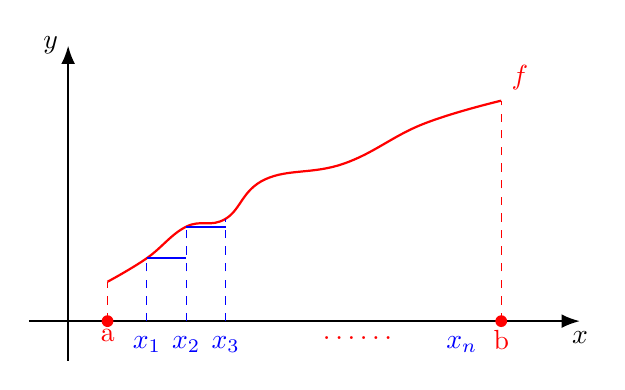
\begin{tikzpicture}[
    >=Latex, % Set default arrow tip style
    axis/.style={->, thick}, % Style for axes
    func/.style={red, thick}, % Style for the function curve
    rect/.style={blue, thick}, % Style for the rectangle
    dashedline/.style={dashed}, % Style for dashed lines
    dot/.style={fill=red, circle, inner sep=1.5pt}, % Style for points a, b
    labelstyle/.style={below=2pt, red} % Style for labels a, x_i, b
]

    % Axes
    \draw[axis] (-0.5, 0) -- (6.5, 0) node[below] {$x$};
    \draw[axis] (0, -0.5) -- (0, 3.5) node[left] {$y$};

    % Function f (approximated with plot smooth)
    \draw[func] plot [smooth, tension=0.7] coordinates {
        (0.5, 0.5) (1.0, 0.8) (1.5, 1.2) (2.0, 1.3) (2.5, 1.8) (3.5, 2.0) (4.5, 2.5) (5.5, 2.8)
    } node[above right] {$f$};

    % Define partition points
    \coordinate (fa) at (0.5,0.5);
    \coordinate (a) at (0.5, 0);
    \coordinate (x1) at (1.0, 0);
    \coordinate (x2) at (1.5, 0);
    \coordinate (x3) at (2.0, 0);
    \coordinate (xn) at (5.0, 0); % Represents x_n
    \coordinate (b) at (5.5, 0);

    % Points and Labels on x-axis
    \node[dot, label={[labelstyle]a}] at (a) {};
    \node[labelstyle, blue] at (x1) {$x_1$};
    \node[labelstyle, blue] at (x2) {$x_2$};
    \node[labelstyle, blue] at (x3) {$x_3$};
    \node[labelstyle, xshift=5pt] at ($(x3)!0.5!(xn)$) {$\dots \dots$}; % Ellipsis between x3 and xn
    \node[labelstyle, blue] at (xn) {$x_n$};
    \node[dot, label={[labelstyle]b}] at (b) {};

    % Dashed lines and Rectangle for Riemann sum approximation
    % Find function values at x1, x2, x3 (approximated from plot coordinates)
    \coordinate (fx1) at (1.0, 0.8);
    \coordinate (fx2) at (1.5, 1.2);
    \coordinate (fx3) at (2.0, 1.3);
    \coordinate (fb)  at (5.5, 2.8); % Function value at b

	
    % Dashed lines from x-axis to function
    \draw[dashedline, red] (a) -- (fa); % Dashed line at b

    \draw[dashedline, blue] (x1) -- (fx1);
    \draw[dashedline, blue] (x2) -- (fx2);
    \draw[dashedline, blue] (x3) -- (fx3);
    \draw[dashedline, red] (b) -- (fb); % Dashed line at b

	\draw[blue, thick] (fx1) -- (1.5,0.8);
	\draw[blue, thick] (fx2) -- (2.0, 1.2);
    % Rectangle using left endpoints (example)
    % Rect 1: width x1-a, height f(a) - approx (0.5,0.5)
    % \draw[rect] (a) rectangle (x1 |- 0.5, 0.5); % Using explicit height
    % Rect 2: width x2-x1, height f(x1)
   % \draw[rect] (x1) rectangle (x2 |- fx1); % Use (coord |- coord) for corner
    % Rect 3: width x3-x2, height f(x2)
   % \draw[rect] (x2) rectangle (x3 |- fx2);

\end{tikzpicture}
\end{document}